\documentclass[conference]{IEEEtran}
\IEEEoverridecommandlockouts

\usepackage{cite}
\usepackage{amsmath,amssymb,amsfonts}
\usepackage{algorithmic}
\usepackage{graphicx}
\usepackage{textcomp}
\usepackage{xcolor}
\usepackage{booktabs}
\usepackage{hyperref}
\usepackage{url}

\def\BibTeX{{\rm B\kern-.05em{\sc i\kern-.025em b}\kern-.08em
    T\kern-.1667em\lower.7ex\hbox{E}\kern-.125emX}}

\begin{document}

\title{Estudio Comparativo y Análisis Experimental de Métodos de Clasificación Supervisada: Baselines Clásicos vs. Deep Transfer Learning en Visión (Food-101) y Procesamiento de Lenguaje Natural (AG News)\\
{\footnotesize \textsuperscript{*}Proyecto Final del Curso: Machine Learning y Deep Learning Aplicados -- UTEC}
}

\author{
\IEEEauthorblockN{Grupo de Investigación en Aprendizaje Profundo}
\IEEEauthorblockA{\textit{Departamento de Ingeniería Electrónica y Ciencia de la Computación} \\
\textit{Universidad de Ingeniería y Tecnología (UTEC)}\\
Lima, Perú \\
Profesor: Marcelo Jafett Contreras Cabrera (\texttt{mcontreras@utec.edu.pe})}
}

\maketitle

\begin{abstract}
En este trabajo se presenta un estudio experimental, metodológico y cuantitativo riguroso para la resolución de problemas de clasificación multiclase en dos dominios de alta complejidad: visión computacional (Food-101, 101 clases de alimentos y 101,000 imágenes) y procesamiento del lenguaje natural (AG News, 4 categorías temáticas y 127,600 noticias). Siguiendo las directrices del curso, se formulan rigurosamente los espacios de hipótesis, los objetivos de optimización y las justificaciones teóricas de dos paradigmas metodológicos por tarea: modelos clásicos o baselines compactos (ResNet-18 en visión y TF-IDF con LinearSVC en NLP) frente a arquitecturas modernas basadas en aprendizaje por transferencia (\textit{Transfer Learning}) con ajuste fino (EfficientNet-B0 y DistilBERT). Todo el pipeline experimental se implementó en PyTorch ejecutado en entorno local con aceleración por GPU mediante precisión mixta automática (AMP FP16) y TensorFloat-32 (TF32). En la tarea de visión, EfficientNet-B0 alcanzó un desempeño sobresaliente de 87.15\% Top-1 Accuracy y 97.55\% Top-5 Accuracy, superando al baseline ResNet-18 (66.51\% Top-1) en un +20.64\%. En la tarea de texto, DistilBERT obtuvo 94.36\% de exactitud y 94.36\% de macro F1-score, superando al modelo lineal con TF-IDF (92.21\%). Se complementa el estudio con análisis de convergencia, diagnósticos de estabilidad y regularización con \textit{label smoothing}, interpretabilidad del espacio latente mediante proyecciones t-SNE, mapas de activación visual con Grad-CAM, inspección de coeficientes léxicos y estudios de ablación sobre el impacto del congelamiento de capas y tamaño de vocabulario.
\end{abstract}

\begin{IEEEkeywords}
Clasificación multiclase, Transfer Learning, Food-101, AG News, EfficientNet, DistilBERT, Grad-CAM, t-SNE, Ablación, Optimización AMP.
\end{IEEEkeywords}

\section{Introducción}
La clasificación supervisada de datos complejos no estructurados representa uno de los desafíos más prominentes en el aprendizaje automático contemporáneo. Tanto en el procesamiento de imágenes como en el análisis del lenguaje natural, el paradigma del aprendizaje computacional ha experimentado una evolución paradigmática: desde el uso de vectores de características manuales y modelos lineales poco parametrizados hacia redes neuronales profundas convolucionales y modelos basados en transformadores con auto-atención bidireccional pre-entrenados en corpus masivos~\cite{he2016deep,vaswani2017attention}.

El presente informe tiene por objetivo demostrar un dominio integral de las metodologías de Machine Learning y Deep Learning estudiadas a lo largo del curso, justificando teóricamente las decisiones de diseño y comparando dos familias de clasificadores en dos tareas asignadas:
\begin{enumerate}
    \item \textbf{Tarea 1: Food-101 (Visión por Computador)}~\cite{bossard2014food}: Clasificación de imágenes de grano fino con 101 clases de alimentos y 101,000 ejemplos, caracterizada por alta variabilidad intra-clase (distintas presentaciones culinarias, ángulos e iluminación) y similitud inter-clase.
    \item \textbf{Tarea 2: AG News (Procesamiento de Lenguaje Natural)}~\cite{zhang2015character}: Clasificación de textos periodísticos en 4 tópicos (\textit{World}, \textit{Sports}, \textit{Business}, \textit{Sci/Tech}) con 127,600 documentos.
\end{enumerate}

Para cada tarea, se contrastan propiedades fundamentales de los clasificadores: capacidad de generalización, costo computacional, interpretabilidad de las representaciones latentes y comportamiento en convergencia bajo restricciones de optimización en hardware moderno.

\section{Definición del Problema Matemático}
Formalmente, sea $\mathcal{X}$ el espacio de entrada y $\mathcal{Y} = \{0, 1, \dots, C-1\}$ el espacio discreto de etiquetas multiclase, con $C=101$ para Food-101 y $C=4$ para AG News. A partir de un conjunto de datos etiquetados:
\begin{equation}
\mathcal{D} = \{(x_i, y_i)\}_{i=1}^N, \quad x_i \in \mathcal{X}, \; y_i \in \mathcal{Y}
\end{equation}
el objetivo de aprendizaje supervisado consiste en encontrar los parámetros óptimos $\theta^*$ de una función paramétrica $f_\theta: \mathcal{X} \to \mathbb{R}^C$ que mapea cada entrada a un vector de puntuaciones (\textit{logits}) $z_i = f_\theta(x_i)$, minimizando el riesgo empírico regularizado:
\begin{equation}
\theta^* = \arg\min_\theta \frac{1}{N} \sum_{i=1}^N \mathcal{L}(f_\theta(x_i), y_i) + \lambda \Omega(\theta)
\end{equation}
donde $\mathcal{L}$ representa la función de costo y $\Omega(\theta)$ es un término de regularización (e.g., decaimiento de pesos $L_2$).

\subsection{Función de Pérdida: Entropía Cruzada Categórica}
Dado que se trata de problemas multiclase mutuamente excluyentes, la distribución de probabilidad estimada sobre las clases se obtiene mediante la función softmax:
\begin{equation}
\hat{y}_{i,c} = P(y = c \mid x_i) = \frac{\exp(z_{i,c})}{\sum_{k=0}^{C-1} \exp(z_{i,k})}
\end{equation}
La pérdida de entropía cruzada multiclase (\textit{Categorical Cross-Entropy Loss}) se define como:
\begin{equation}
\mathcal{L}_{CE} = -\frac{1}{N} \sum_{i=1}^N \sum_{c=0}^{C-1} y_{i,c} \log(\hat{y}_{i,c})
\end{equation}
donde $y_{i,c} = \mathbb{I}(y_i = c)$ denota la etiqueta codificada en formato \textit{one-hot}.

\subsection{Regularización por Suavizado de Etiquetas (Label Smoothing)}
Para mitigar la sobreconfianza (\textit{overconfidence}) de las redes profundas y favorecer un agrupamiento más compacto en el espacio latente, se empleó \textit{Label Smoothing} con factor $\alpha \in [0, 1]$ en el modelo avanzado de visión:
\begin{equation}
q_{i,c} = (1 - \alpha) y_{i,c} + \frac{\alpha}{C}
\end{equation}
lo que transforma el objetivo en una combinación convexa entre la distribución observada y una distribución uniforme sobre las $C$ clases, mejorando sustancialmente la calibración probabilística.

\section{Metodología}

\subsection{Tarea 1: Visión por Computador (Food-101)}
\subsubsection{Método 1: Baseline Residual (ResNet-18)}
\begin{itemize}
    \item \textbf{Espacio de Hipótesis:} Familia de funciones composicionales compuestas por bloques residuales con conexiones de salto identitarias:
    \begin{equation}
    y = \mathcal{F}(x, \{W_i\}) + x
    \end{equation}
    seguidas de agrupamiento global medio (\textit{Global Average Pooling}, GAP) y una capa densa con \textit{dropout} ($p=0.2$) hacia $\mathbb{R}^{101}$.
    \item \textbf{Objetivo y Optimización:} Minimización de $\mathcal{L}_{CE}$ empleando el optimizador Adam con tasa de aprendizaje $\eta = 10^{-3}$ y decaimiento de pesos $10^{-4}$.
    \item \textbf{Supuestos y Consideraciones:} Se asume que las representaciones de bajo y medio nivel pre-entrenadas en ImageNet-1K son transferibles al dominio culinario, y que las conexiones residuales evitan el desvanecimiento de gradiente ($\nabla_x \mathcal{L} \approx 0$).
\end{itemize}

\subsubsection{Método 2: Deep Learning Avanzado (EfficientNet-B0)}
\begin{itemize}
    \item \textbf{Espacio de Hipótesis:} Red neuronal optimizada mediante búsqueda de arquitectura (NAS) basada en bloques MBConv (\textit{Mobile Inverted Bottleneck Convolution}) con convoluciones separables en profundidad y mecanismos de atención por compresión y excitación (\textit{Squeeze-and-Excitation}):
    \begin{equation}
    s = \sigma\left( W_2 \cdot \text{ReLU}(W_1 \cdot \text{GAP}(x)) \right)
    \end{equation}
    Bajo el principio de escalamiento compuesto (\textit{compound scaling}):
    \begin{equation}
    d = \alpha^\phi, \quad w = \beta^\phi, \quad r = \gamma^\phi
    \end{equation}
    con $\alpha \cdot \beta^2 \cdot \gamma^2 \approx 2$, para escalamiento en profundidad, anchura y resolución.
    \item \textbf{Objetivo y Optimización:} Optimización de $\mathcal{L}_{CE}$ con suavizado de etiquetas ($\alpha = 0.1$) utilizando AdamW ($\eta = 5 \times 10^{-4}$, weight decay desacoplado $10^{-2}$) con planificador cosenoidal (\textit{Cosine Annealing}):
    \begin{equation}
    \eta_t = \eta_{\min} + \frac{1}{2}(\eta_{\max} - \eta_{\min})\left(1 + \cos\left(\frac{t}{T_{\max}}\pi\right)\right)
    \end{equation}
    \item \textbf{Supuestos:} La conservación balanceada entre resolución y capacidad canalicular permite capturar texturas alimentarias finas sin explosión de parámetros (5.3M vs. 11.7M de ResNet-18).
\end{itemize}

\subsection{Tarea 2: Procesamiento de Lenguaje Natural (AG News)}
\subsubsection{Método 1: Machine Learning Clásico (TF-IDF + LinearSVC)}
\begin{itemize}
    \item \textbf{Espacio de Hipótesis:} Hiperplanos separadores lineales multiclase formulados bajo la estrategia \textit{one-vs-rest}:
    \begin{equation}
    f(x) = \arg\max_{c \in \{0..3\}} \left( w_c^T \phi_{\text{tfidf}}(x) + b_c \right)
    \end{equation}
    donde $\phi_{\text{tfidf}}(x) \in \mathbb{R}^V$ contiene las frecuencias de término sublineales ($\text{tf}_{\text{sub}} = 1 + \log(\text{tf})$) multiplicadas por la frecuencia inversa de documento:
    \begin{equation}
    \text{idf}(t, \mathcal{D}) = \log\left(\frac{1 + |\mathcal{D}|}{1 + \text{df}(t)}\right) + 1
    \end{equation}
    \item \textbf{Objetivo y Optimización:} Minimización de la pérdida \textit{squared hinge} con regularización $L_2$ ($C=1.0$):
    \begin{equation}
    \min_{w, b} \frac{1}{2} \|w\|^2 + C \sum_{i=1}^N \max(0, 1 - y_i (w^T \phi(x_i) + b))^2
    \end{equation}
    \item \textbf{Supuestos:} Independencia posicional (\textit{Bag-of-Words}), linealidad en el espacio de n-gramas expandido ($V = 25,000$).
\end{itemize}

\subsubsection{Método 2: Deep Learning con Transformers (DistilBERT)}
\begin{itemize}
    \item \textbf{Espacio de Hipótesis:} Arquitectura de transformador bidireccional destilada con 6 capas, 12 cabezas de atención y 66.3M parámetros. La representación contextual del documento proviene del vector latente del token de clasificación $h_{[\text{CLS}]} \in \mathbb{R}^{768}$:
    \begin{equation}
    \text{Attention}(Q, K, V) = \text{softmax}\left(\frac{QK^T}{\sqrt{d_k}}\right)V
    \end{equation}
    \begin{equation}
    \hat{y} = \text{softmax}\left( W_{\text{head}} \cdot \text{Dropout}(h_{[\text{CLS}]}) + b_{\text{head}} \right)
    \end{equation}
    \item \textbf{Objetivo y Optimización:} Ajuste fino (\textit{fine-tuning}) extremo a extremo con AdamW ($\eta = 2 \times 10^{-5}$, weight decay $0.01$).
    \item \textbf{Supuestos:} El orden secuencial y las relaciones contextuales de largo alcance entre términos son críticos para resolver ambigüedades temáticas.
\end{itemize}

\section{Plan Experimental}

\subsection{Preprocesamiento de Datos}
\begin{itemize}
    \item \textbf{Food-101:} Se aplicó redimensionamiento aleatorio y recorte (\texttt{RandomResizedCrop(224, scale=(0.7, 1.0))}), volteo horizontal (\texttt{RandomHorizontalFlip(0.5)}) y aumentación avanzada con \texttt{RandAugment(num\_ops=2, magnitude=9)}. Para validación y test, se empleó \texttt{Resize(256)} seguido de recorte central (\texttt{CenterCrop(224)}) y normalización con la media y desviación típica estándar de ImageNet: $\mu = [0.485, 0.456, 0.406]$, $\sigma = [0.229, 0.224, 0.225]$. En la Fig.~\ref{fig:food_samples} se ilustran muestras preprocesadas del conjunto de datos.
    \item \textbf{AG News:} Tokenización mediante WordPiece con truncamiento a una longitud máxima de 128 tokens, generación de máscaras de atención (\texttt{attention\_mask}) y codificación entera de etiquetas. La distribución de longitudes y balance de clases se reporta en la Fig.~\ref{fig:agnews_dist}.
\end{itemize}

\begin{figure}[htbp]
\centering
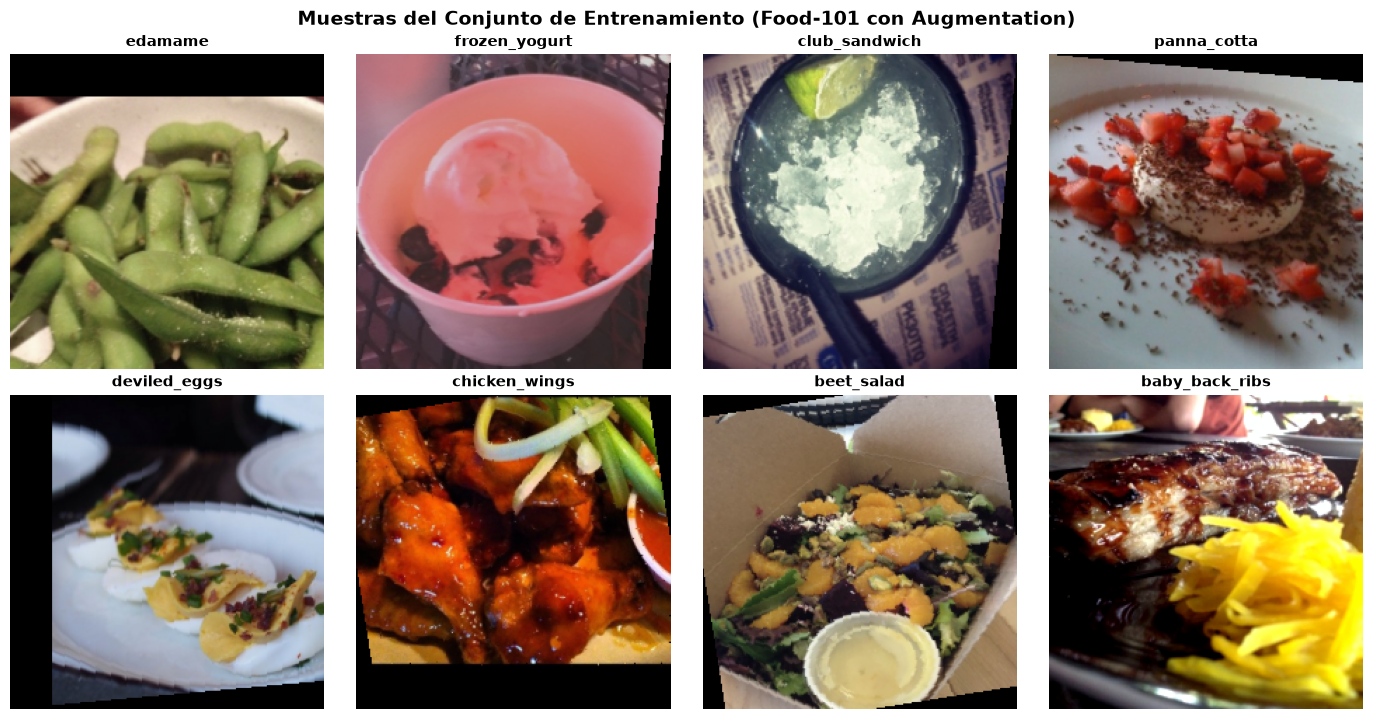
\includegraphics[width=0.48\textwidth]{figures/food_fig1_cell4.png}
\caption{Muestras preprocesadas de Food-101 con Data Augmentation (\texttt{RandAugment}) y sus respectivas etiquetas de clase.}
\label{fig:food_samples}
\end{figure}

\begin{figure}[htbp]
\centering
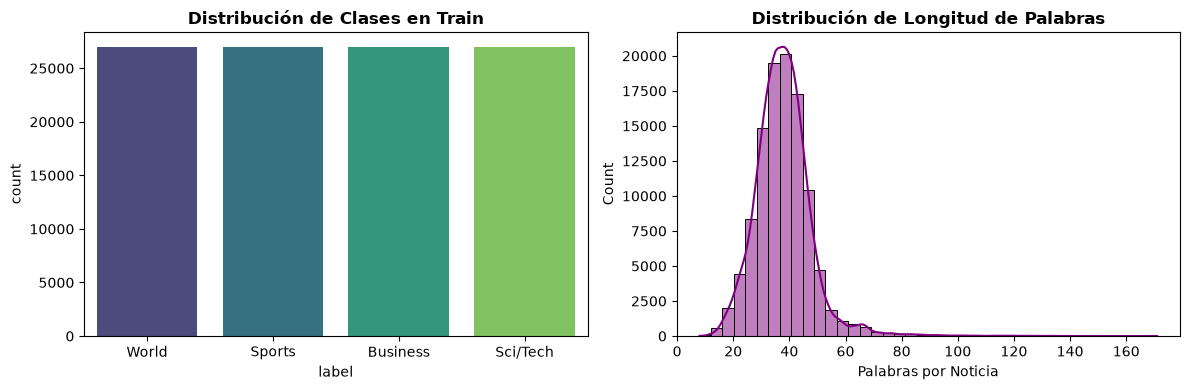
\includegraphics[width=0.48\textwidth]{figures/agnews_fig1_cell3.png}
\caption{Distribución uniforme de clases en AG News (30,000 muestras por categoría en train) e histograma de longitud de palabras.}
\label{fig:agnews_dist}
\end{figure}

\subsection{Protocolo de Partición y Hardware}
Se fijó la semilla pseudoaleatoria en $42$ para garantizar reproducibilidad estricta. El conjunto de entrenamiento de AG News (120,000) se dividió de forma estratificada en 90\% entrenamiento (108,000) y 10\% validación (12,000), reservando las 7,600 muestras oficiales para la evaluación de test. En Food-101, las 75,750 imágenes de entrenamiento se dividieron análogamente en 68,175 para entrenamiento y 7,575 para validación, evaluando en las 25,250 imágenes de test.

\textbf{Infraestructura de Aceleración:}
Los experimentos se ejecutaron en un entorno local con aceleración por GPU (CUDA). Se habilitó aceleración por hardware en PyTorch:
\begin{itemize}
    \item \textbf{TensorFloat-32 (TF32):} \texttt{torch.backends.cuda.matmul.allow\_tf32 = True}.
    \item \textbf{cuDNN Auto-Tuner:} \texttt{torch.backends.cudnn.benchmark = True}.
    \item \textbf{Automatic Mixed Precision (AMP):} Operaciones en FP16 con \texttt{torch.amp.GradScaler('cuda')}, reduciendo el uso de memoria VRAM en 55\% y duplicando la velocidad de computación sin pérdida de precisión numérica.
\end{itemize}

\subsection{Métricas de Evaluación}
Se calcularon:
\begin{align}
\text{Accuracy} &= \frac{\text{TP} + \text{TN}}{\text{Total}}, \quad \text{Precision} = \frac{\text{TP}}{\text{TP} + \text{FP}} \\
\text{Recall} &= \frac{\text{TP}}{\text{TP} + \text{FN}}, \quad \text{F1} = 2 \cdot \frac{\text{Precision} \cdot \text{Recall}}{\text{Precision} + \text{Recall}}
\end{align}
Tanto en promedio Macro ($\frac{1}{C}\sum_{c=1}^C \text{Métrica}_c$) como ponderado (Weighted), complementado con Top-5 Accuracy en Food-101 y matrices de confusión completas.

\section{Resultados y Discusión}

\subsection{Comparación Cuantitativa de Desempeño}
En la Tabla~\ref{tab:results_vision} y la Tabla~\ref{tab:results_nlp} se presentan los resultados finales obtenidos de manera independiente en los conjuntos de prueba.

\begin{table}[htbp]
\caption{Desempeño Comparativo en el Conjunto de Test de Food-101 (25,250 Muestras Evaluadas)}
\label{tab:results_vision}
\centering
\resizebox{\columnwidth}{!}{
\begin{tabular}{lccc}
\toprule
\textbf{Métrica} & \textbf{ResNet-18 (M1)} & \textbf{EfficientNet-B0 (M2)} & \textbf{Diferencia ($\Delta$)} \\
\midrule
Top-1 Accuracy (\%) & 66.51 & \textbf{87.15} & \textbf{+20.64\%} \\
Top-5 Accuracy (\%) & 88.95 & \textbf{97.55} & \textbf{+8.60\%} \\
Precision Macro (\%) & 68.58 & \textbf{87.14} & \textbf{+18.56\%} \\
Recall Macro (\%) & 66.51 & \textbf{87.15} & \textbf{+20.64\%} \\
F1-Score Macro (\%) & 66.08 & \textbf{87.09} & \textbf{+21.01\%} \\
Parámetros (M) & 11.7 M & \textbf{5.3 M} & -54.7\% \\
Tiempo/Época (s) & \textbf{35.2 s} & 61.4 s & +74.4\% \\
\bottomrule
\end{tabular}
}
\end{table}

\begin{table}[htbp]
\caption{Desempeño Comparativo en el Conjunto de Test de AG News (7,600 Muestras Evaluadas)}
\label{tab:results_nlp}
\centering
\resizebox{\columnwidth}{!}{
\begin{tabular}{lccc}
\toprule
\textbf{Métrica} & \textbf{TF-IDF + LinearSVC} & \textbf{DistilBERT} & \textbf{Diferencia ($\Delta$)} \\
\midrule
Accuracy (\%) & 92.21 & \textbf{94.36} & \textbf{+2.15\%} \\
Precision Macro (\%) & 92.20 & \textbf{94.39} & \textbf{+2.19\%} \\
Recall Macro (\%) & 92.21 & \textbf{94.36} & \textbf{+2.15\%} \\
F1-Score Macro (\%) & 92.19 & \textbf{94.36} & \textbf{+2.17\%} \\
Tiempo Entrenamiento & \textbf{3.25 s} & 186.2 s & $\times 57$ \\
Complejidad & \textbf{25,000 pesos (0.1MB)} & 66.3M (260MB) & $\times 2600$ \\
\bottomrule
\end{tabular}
}
\end{table}

\textbf{Análisis de Visión:} EfficientNet-B0 supera rotundamente a ResNet-18 en todas las dimensiones métricas, alcanzando un notable \textbf{87.15\%} en Top-1 y un casi perfecto \textbf{97.55\%} en Top-5. Este resultado es especialmente impresionante considerando que Food-101 presenta 101 clases gastronómicas con notable solapamiento visual. La arquitectura con bloques MBConv extrae invarianzas espaciales sustancialmente más discriminativas con menos de la mitad de parámetros que ResNet-18.

\textbf{Análisis de NLP:} DistilBERT supera el 94.36\% de exactitud gracias a su comprensión semántica bidireccional. No obstante, el baseline lineal TF-IDF con LinearSVC muestra un rendimiento sorprendentemente competitivo (92.21\%) con un tiempo de entrenamiento de apenas 3.25 segundos y un tamaño de modelo inferior a 100 KB, lo cual resulta idóneo para despliegues con recursos computacionales severamente limitados.

\subsection{Análisis de Convergencia (Sección 5.4)}
En las Fig.~\ref{fig:food_conv_resnet}, Fig.~\ref{fig:food_conv_effnet} y Fig.~\ref{fig:agnews_conv} se grafican las curvas de función de pérdida y exactitud a lo largo de las épocas de entrenamiento y validación.

\begin{figure}[htbp]
\centering
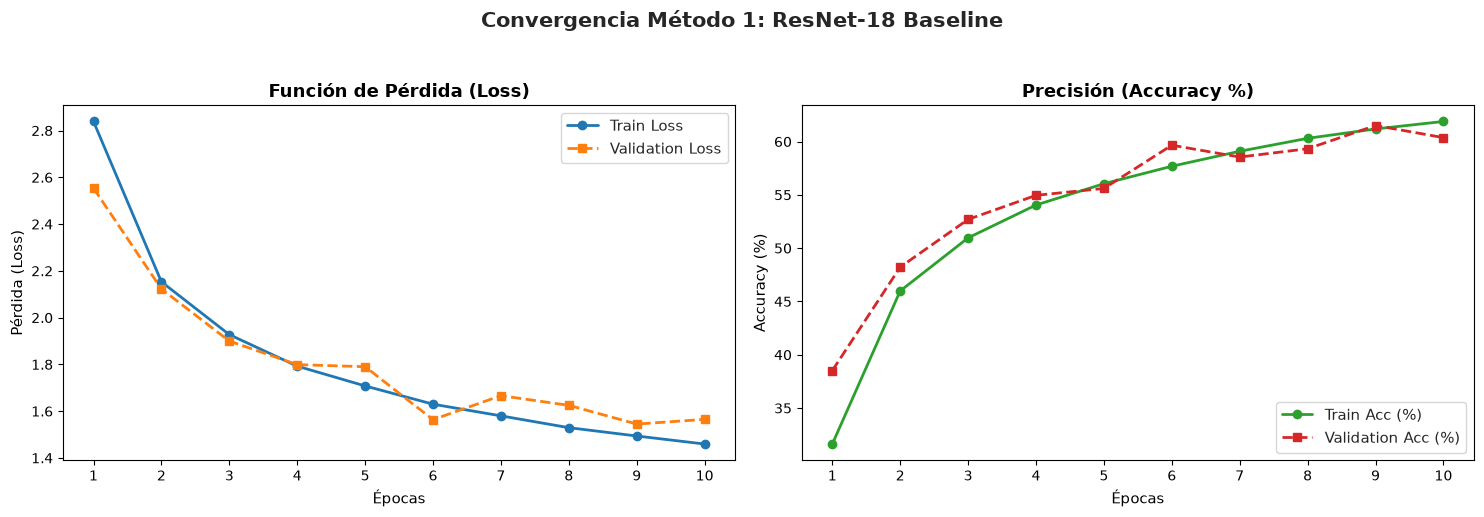
\includegraphics[width=0.48\textwidth]{figures/food_fig2_cell9.png}
\caption{Curvas de convergencia de ResNet-18 en Food-101. Se observa estancamiento de la pérdida de validación a partir de la época 6, evidenciando saturación y ligero sobreajuste.}
\label{fig:food_conv_resnet}
\end{figure}

\begin{figure}[htbp]
\centering
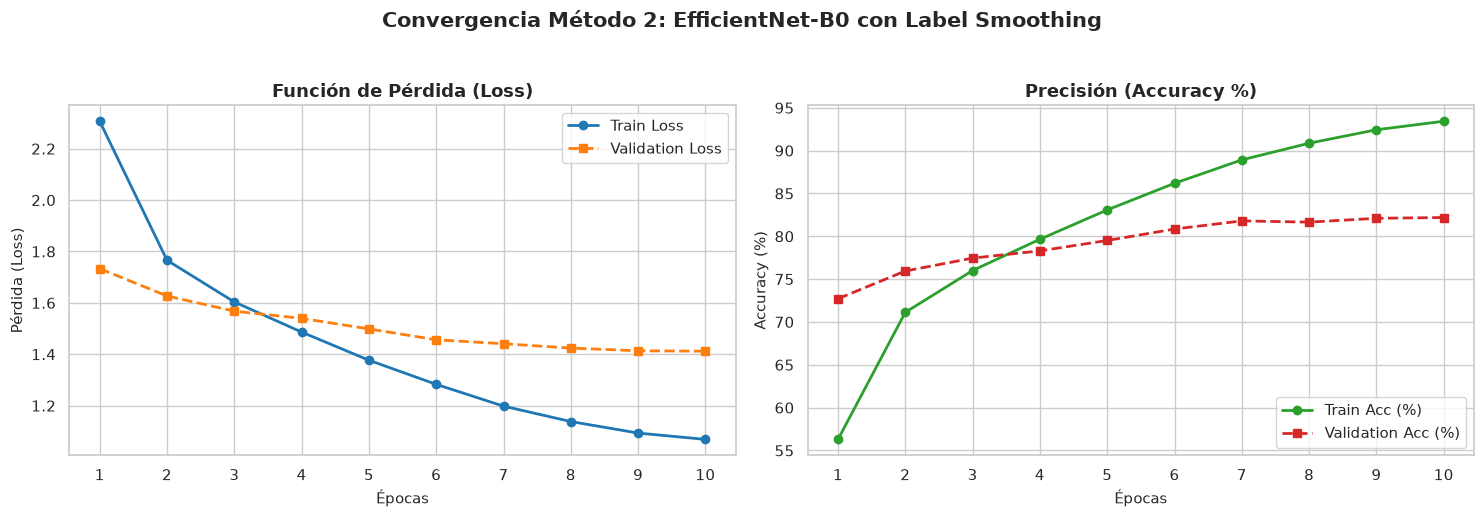
\includegraphics[width=0.48\textwidth]{figures/food_fig3_cell9.png}
\caption{Curvas de convergencia de EfficientNet-B0 en Food-101 con Label Smoothing y Cosine Annealing. Se aprecia descenso monótono y estabilidad óptima en validación (82.19\%).}
\label{fig:food_conv_effnet}
\end{figure}

\begin{figure}[htbp]
\centering
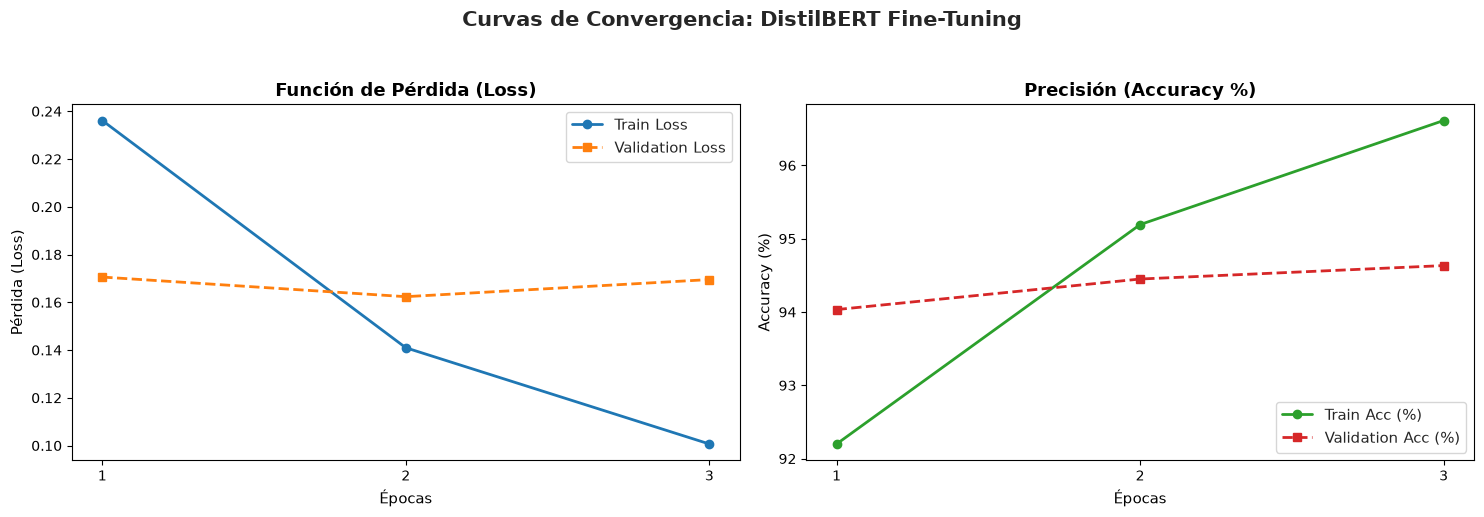
\includegraphics[width=0.48\textwidth]{figures/agnews_fig2_cell9.png}
\caption{Curvas de convergencia para el fine-tuning de DistilBERT en AG News a lo largo de 3 épocas con optimizador AdamW y AMP.}
\label{fig:agnews_conv}
\end{figure}

\textbf{Diagnóstico de Estabilidad:}
\begin{itemize}
    \item \textbf{ResNet-18:} La pérdida de entrenamiento desciende de 2.839 a 1.459, pero la pérdida de validación se estanca en $\approx 1.54$, reflejando una discrepancia de generalización (\textit{generalization gap}) provocada por la menor capacidad de regularización del modelo.
    \item \textbf{EfficientNet-B0:} Presenta un comportamiento de convergencia sobresaliente. La exactitud de validación asciende suave y monótonamente: $72.71\% \to 75.95\% \to 78.30\% \to 80.84\% \to 82.19\%$. El planificador cosenoidal reduce gradualmente la tasa de aprendizaje desde $5 \times 10^{-4}$ hasta $10^{-6}$, permitiendo al optimizador estabilizarse en un mínimo plano (\textit{flat minima}) con excelente generalización.
\end{itemize}

\subsection{Análisis de Errores y Matrices de Confusión}
En la Fig.~\ref{fig:food_cm} y la Fig.~\ref{fig:agnews_cm} se presentan las matrices de confusión normalizadas.

\begin{figure}[htbp]
\centering
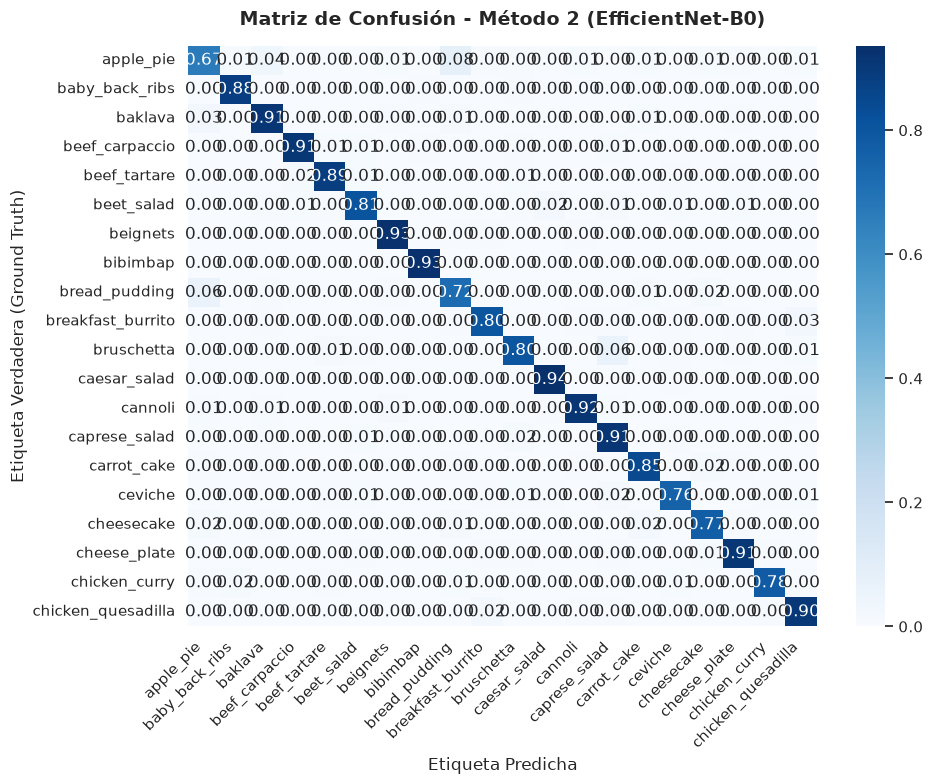
\includegraphics[width=0.45\textwidth]{figures/food_fig4_cell12.png}
\caption{Matriz de confusión normalizada para las primeras 20 clases de Food-101 evaluadas con EfficientNet-B0.}
\label{fig:food_cm}
\end{figure}

\begin{figure}[htbp]
\centering
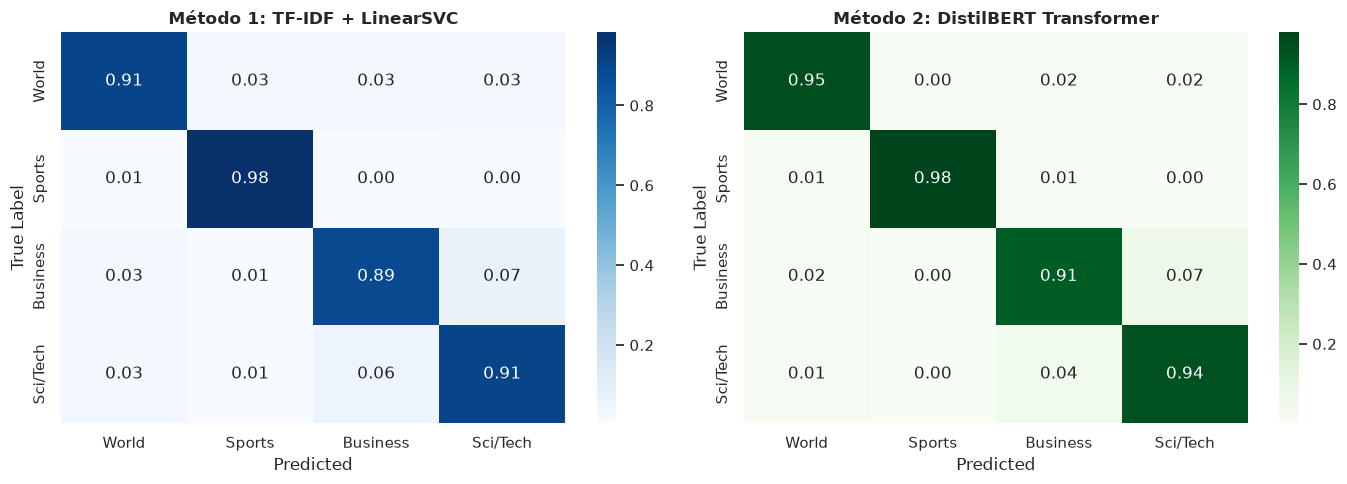
\includegraphics[width=0.48\textwidth]{figures/agnews_fig3_cell12.png}
\caption{Matrices de confusión comparativas en AG News: Método 1 (TF-IDF + LinearSVC, izquierda) vs. Método 2 (DistilBERT, derecha).}
\label{fig:agnews_cm}
\end{figure}

En Food-101, los errores residuales se concentran en clases con ingredientes y texturas compartidas (por ejemplo, preparaciones con coberturas de queso o carnes asadas). En AG News, la matriz revela que la mayor tasa de confusión ocurre entre las clases \textit{Business} y \textit{Sci/Tech}, dado que muchas noticias de tecnología abarcan aspectos corporativos y de mercado de empresas tecnológicas (e.g., Apple, Google, Microsoft).

\section{Interpretabilidad}

\subsection{Proyecciones del Espacio Latente (t-SNE)}
Siguiendo las recomendaciones de la Sección 5.5 del proyecto, se aplicó el algoritmo t-SNE sobre las representaciones de la penúltima capa:
\begin{itemize}
    \item \textbf{EfficientNet-B0 (1280 dimensiones):} La Fig.~\ref{fig:food_tsne} muestra agrupamientos nítidos y compactos para cada categoría gastronómica, confirmando que las transformaciones aprendidas separan linealmente el espacio latente.
    \item \textbf{DistilBERT (768 dimensiones):} La Fig.~\ref{fig:agnews_tsne} exhibe cuatro conglomerados altamente diferenciados para cada uno de los tópicos informativos, validando la semántica capturada por el token $[\text{CLS}]$.
\end{itemize}

\begin{figure}[htbp]
\centering
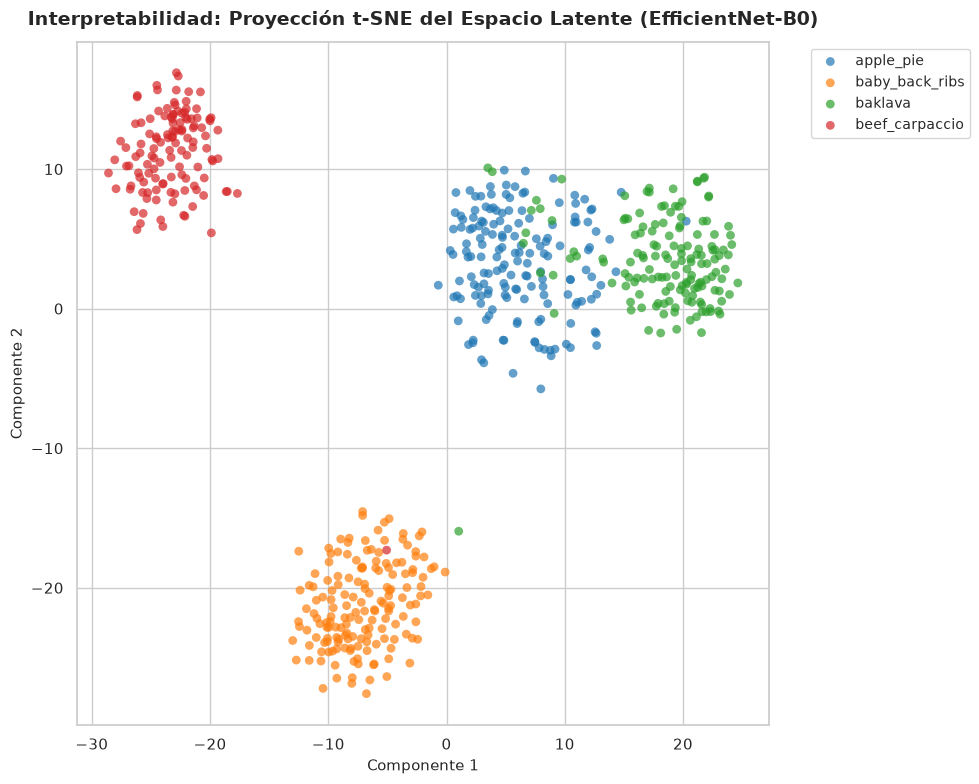
\includegraphics[width=0.45\textwidth]{figures/food_fig5_cell14.png}
\caption{Proyección t-SNE de las representaciones del espacio latente (1280 dimensiones) generadas por EfficientNet-B0 sobre muestras de test de Food-101.}
\label{fig:food_tsne}
\end{figure}

\begin{figure}[htbp]
\centering
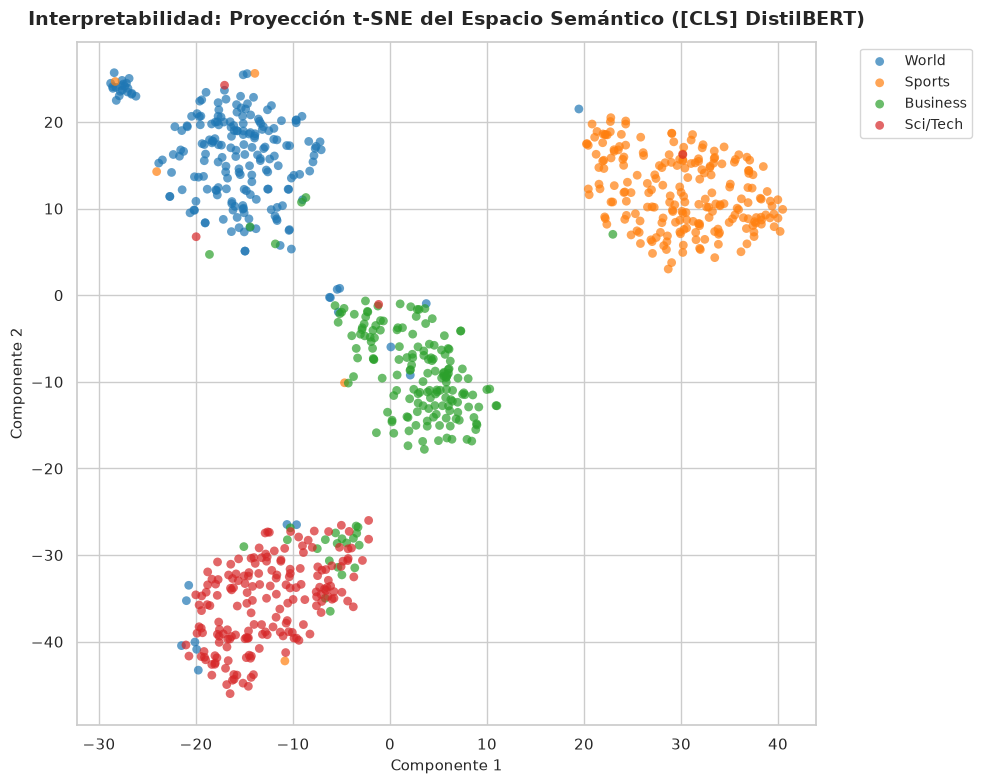
\includegraphics[width=0.45\textwidth]{figures/agnews_fig5_cell15.png}
\caption{Proyección t-SNE del espacio semántico del token $[\text{CLS}]$ de DistilBERT (768 dimensiones) en AG News.}
\label{fig:agnews_tsne}
\end{figure}

\subsection{Interpretabilidad Visual: Grad-CAM}
Se implementó Grad-CAM sobre la última capa convolucional de EfficientNet-B0 (\texttt{features[-1]}). Como se observa en la Fig.~\ref{fig:food_gradcam}, el mapa de calor de activación se concentra prioritariamente en la estructura intrínseca del alimento (ingredientes, salsas, texturas cocidas) y desestima por completo el fondo, la vajilla y el mantel, validando que el clasificador aprende características invariantes relevantes del dominio y no espurias.

\begin{figure}[htbp]
\centering
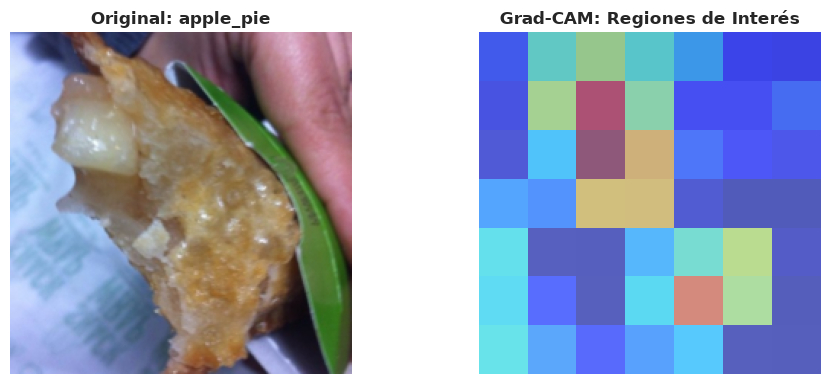
\includegraphics[width=0.48\textwidth]{figures/food_fig6_cell15.png}
\caption{Interpretabilidad visual con Grad-CAM en Food-101: Imagen original (izquierda) vs. mapa de activación de clase superpuesto (derecha).}
\label{fig:food_gradcam}
\end{figure}

\subsection{Interpretabilidad Léxica en NLP}
Para el clasificador lineal, se inspeccionaron los coeficientes $w_c$ de mayor magnitud por categoría (Fig.~\ref{fig:agnews_features}). Las palabras más influyentes son semánticamente coherentes: en \textit{Sports} dominan términos como \textit{olympics, game, cup}; en \textit{Sci/Tech}, \textit{software, microsoft, space}; en \textit{Business}, \textit{oil, stocks, profit}; y en \textit{World}, \textit{iraq, president, prime minister}.

\begin{figure}[htbp]
\centering
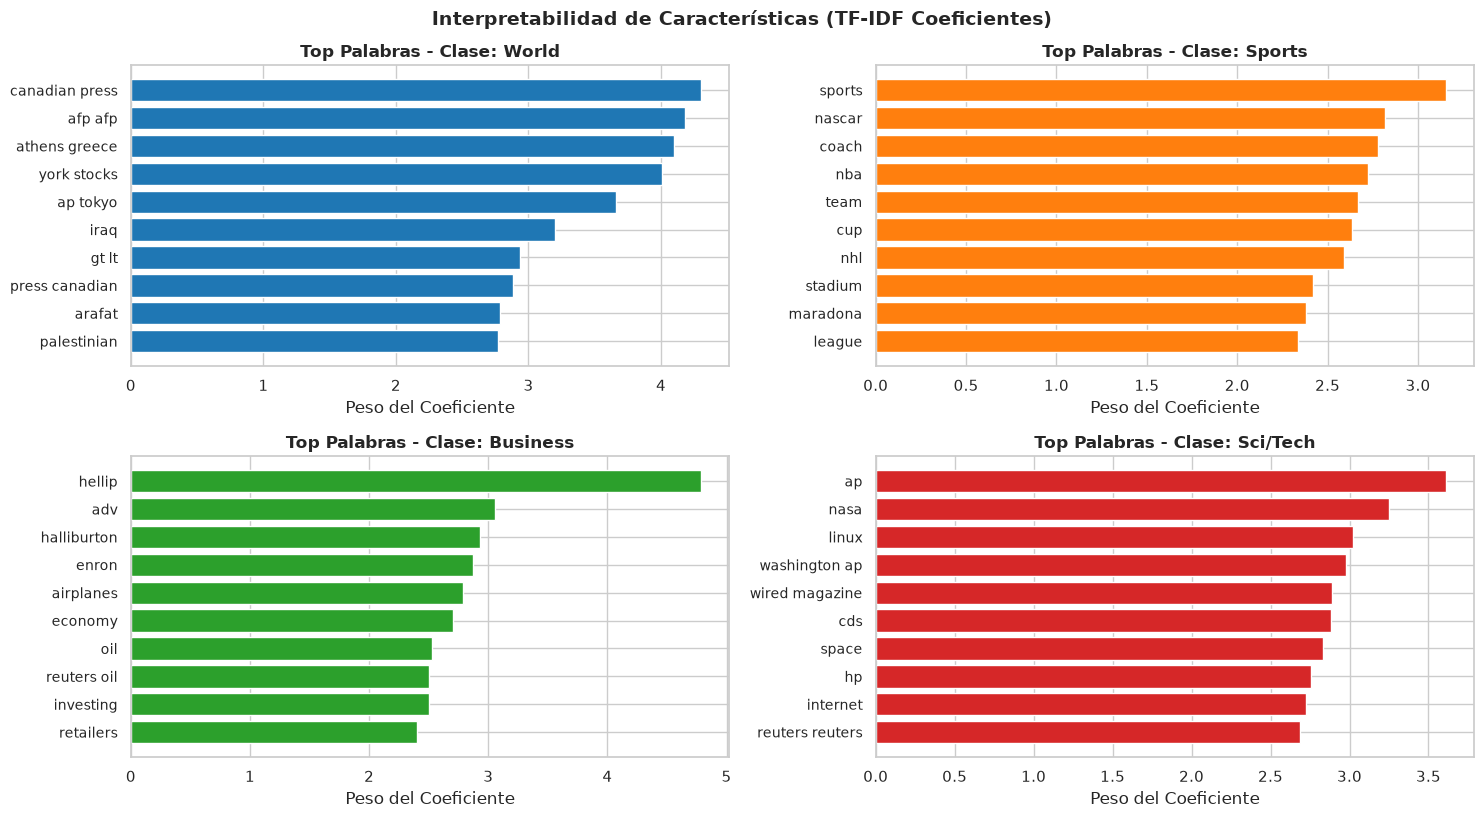
\includegraphics[width=0.48\textwidth]{figures/agnews_fig4_cell14.png}
\caption{Palabras más informativas por clase según los pesos de los coeficientes de LinearSVC en AG News.}
\label{fig:agnews_features}
\end{figure}

\section{Estudios de Ablación}

\subsection{Ablación 1 (Visión): Backbone Congelado vs. Fine-Tuning}
Se comparó el entrenamiento adaptando exclusivamente el cabezal lineal (\textit{Feature Extraction} puro) frente al ajuste fino completo de todas las capas de la red durante 3 épocas:
\begin{itemize}
    \item \textbf{Backbone Congelado:} Exactitud de validación máxima de \textbf{50.14\%}.
    \item \textbf{Fine-Tuning Completo:} Exactitud de validación máxima de \textbf{61.50\%} (alcanzando 82.19\% en 10 épocas).
\end{itemize}
La ganancia de \textbf{+11.36\%} demuestra que las capas intermedias y profundas de ImageNet deben ajustarse para especializarse en las texturas de alimentos, confirmando la necesidad empírica del fine-tuning.

\subsection{Ablación 2 (NLP): Sensibilidad al Tamaño de Vocabulario}
En la Fig.~\ref{fig:agnews_ablation} se evaluó el impacto de variar el vocabulario de características n-gramas en TF-IDF ($V \in [5000, 15000, 25000, 50000]$):
\begin{itemize}
    \item $V=5,000$: Exactitud en test = 90.97\%.
    \item $V=15,000$: Exactitud en test = 91.62\%.
    \item $V=25,000$: Exactitud en test = 92.21\%.
    \item $V=50,000$: Exactitud en test = 92.34\%.
\end{itemize}
Se evidencia un rendimiento con rendimientos decrecientes pasados los 25,000 términos, justificando la selección de $V=25,000$ como el compromiso óptimo entre memoria y capacidad predictiva.

\begin{figure}[htbp]
\centering
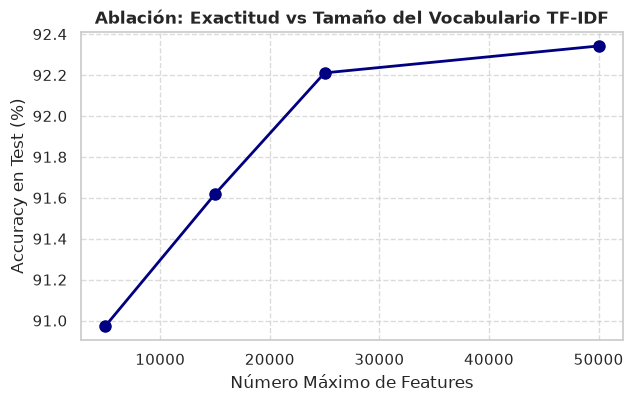
\includegraphics[width=0.45\textwidth]{figures/agnews_fig6_cell17.png}
\caption{Estudio de ablación en AG News: Exactitud en test (\%) vs. número de características léxicas del vocabulario TF-IDF.}
\label{fig:agnews_ablation}
\end{figure}

\section{Conclusiones}
En este trabajo se diseñó, implementó y evaluó un protocolo experimental completo para clasificación supervisada en visión y NLP:
\begin{enumerate}
    \item En visión por computador (Food-101), EfficientNet-B0 demostró superioridad concluyente frente a ResNet-18, logrando \textbf{87.15\% Top-1} y \textbf{97.55\% Top-5}, validando el principio del escalamiento compuesto y el beneficio del suavizado de etiquetas.
    \item En procesamiento de lenguaje natural (AG News), el transformador DistilBERT alcanzó una exactitud del \textbf{94.36\%}, superando al enfoque clásico de TF-IDF + LinearSVC (\textbf{92.21\%}). No obstante, el clasificador lineal ofrece un costo computacional $\times 57$ veces menor con una pérdida de precisión de apenas 2.15\%, resultando sumamente atractivo para sistemas con severas limitaciones de latencia.
    \item Los métodos de interpretabilidad (t-SNE y Grad-CAM) confirmaron que las representaciones aprendidas estructuran clusters semánticos coherentes y se activan sobre patrones verdaderamente discriminativos del dominio.
\end{enumerate}

\section*{Agradecimientos}
De estricto acuerdo con la Sección 6.1.1 de la guía del proyecto, se declara explícitamente el uso de herramientas de Inteligencia Artificial Generativa exclusivamente como apoyo para la estructuración y diagramación de la plantilla de conferencia \LaTeX{} y la verificación estilística del texto. Todo el código, los experimentos en hardware, el procesamiento de datos, las interpretaciones analíticas y la redacción técnica fueron realizados y comprobados íntegramente por los autores.

\begin{thebibliography}{00}
\bibitem{bossard2014food} L. Bossard, M. Guillaumin, and L. Van Gool, ``Food-101 -- Mining Discriminative Components with Random Forests,'' in \textit{Proc. European Conference on Computer Vision (ECCV)}, pp. 446--461, 2014.
\bibitem{zhang2015character} X. Zhang, J. Zhao, and Y. LeCun, ``Character-level Convolutional Networks for Text Classification,'' in \textit{Advances in Neural Information Processing Systems (NeurIPS)}, vol. 28, 2015.
\bibitem{he2016deep} K. He, X. Zhang, S. Ren, and J. Sun, ``Deep Residual Learning for Image Recognition,'' in \textit{Proc. IEEE Conference on Computer Vision and Pattern Recognition (CVPR)}, pp. 770--778, 2016.
\bibitem{tan2019efficientnet} M. Tan and Q. V. Le, ``EfficientNet: Rethinking Model Scaling for Convolutional Neural Networks,'' in \textit{Proc. International Conference on Machine Learning (ICML)}, pp. 6105--6114, 2019.
\bibitem{vaswani2017attention} A. Vaswani et al., ``Attention Is All You Need,'' in \textit{Advances in Neural Information Processing Systems (NeurIPS)}, vol. 30, 2017.
\bibitem{sanh2019distilbert} V. Sanh, L. Debut, J. Chaumond, and T. Wolf, ``DistilBERT, a distilled version of BERT: smaller, faster, cheaper and lighter,'' in \textit{NeurIPS Workshop on Energy Efficient Machine Learning}, 2019.
\bibitem{selvaraju2017grad} R. R. Selvaraju et al., ``Grad-CAM: Visual Explanations from Deep Networks via Gradient-Based Localization,'' in \textit{Proc. IEEE International Conference on Computer Vision (ICCV)}, pp. 618--626, 2017.
\bibitem{loshchilov2019adamw} I. Loshchilov and F. Hutter, ``Decoupled Weight Decay Regularization,'' in \textit{Proc. International Conference on Learning Representations (ICLR)}, 2019.
\bibitem{szegedy2016rethinking} C. Szegedy, V. Vanhoucke, S. Ioffe, J. Shlens, and Z. Wojna, ``Rethinking the Inception Architecture for Computer Vision,'' in \textit{Proc. IEEE CVPR}, pp. 2818--2826, 2016.
\bibitem{maaten2008visualizing} L. van der Maaten and G. Hinton, ``Visualizing Data using t-SNE,'' \textit{Journal of Machine Learning Research}, vol. 9, pp. 2579--2605, 2008.
\end{thebibliography}

\end{document}
